\section{ASZ Architecture and Tuning Granularity}
\label{sec:overview}

ASZ retains the two-stage organization of the SZ pipeline, preprocessing followed by compression, but changes how it predicts and serializes data and how it chooses the corresponding configurations. During compression, ASZ predicts each round along its own selected axis, selects the coefficients of its four-reference predictor separately for each data block, and serializes the QBs of each round in a selectable order. During preprocessing, ASZ determines these round-wise choices using reverse-greedy search with fast evaluation of candidate configurations. It records them in a configuration plan, which specifies one prediction stencil for the entire field, together with one prediction axis and one QB serialization order for each round. Fig.~\ref{fig:overview:asz-workflow} summarizes this workflow.

\begin{figure}[htb]
\centering
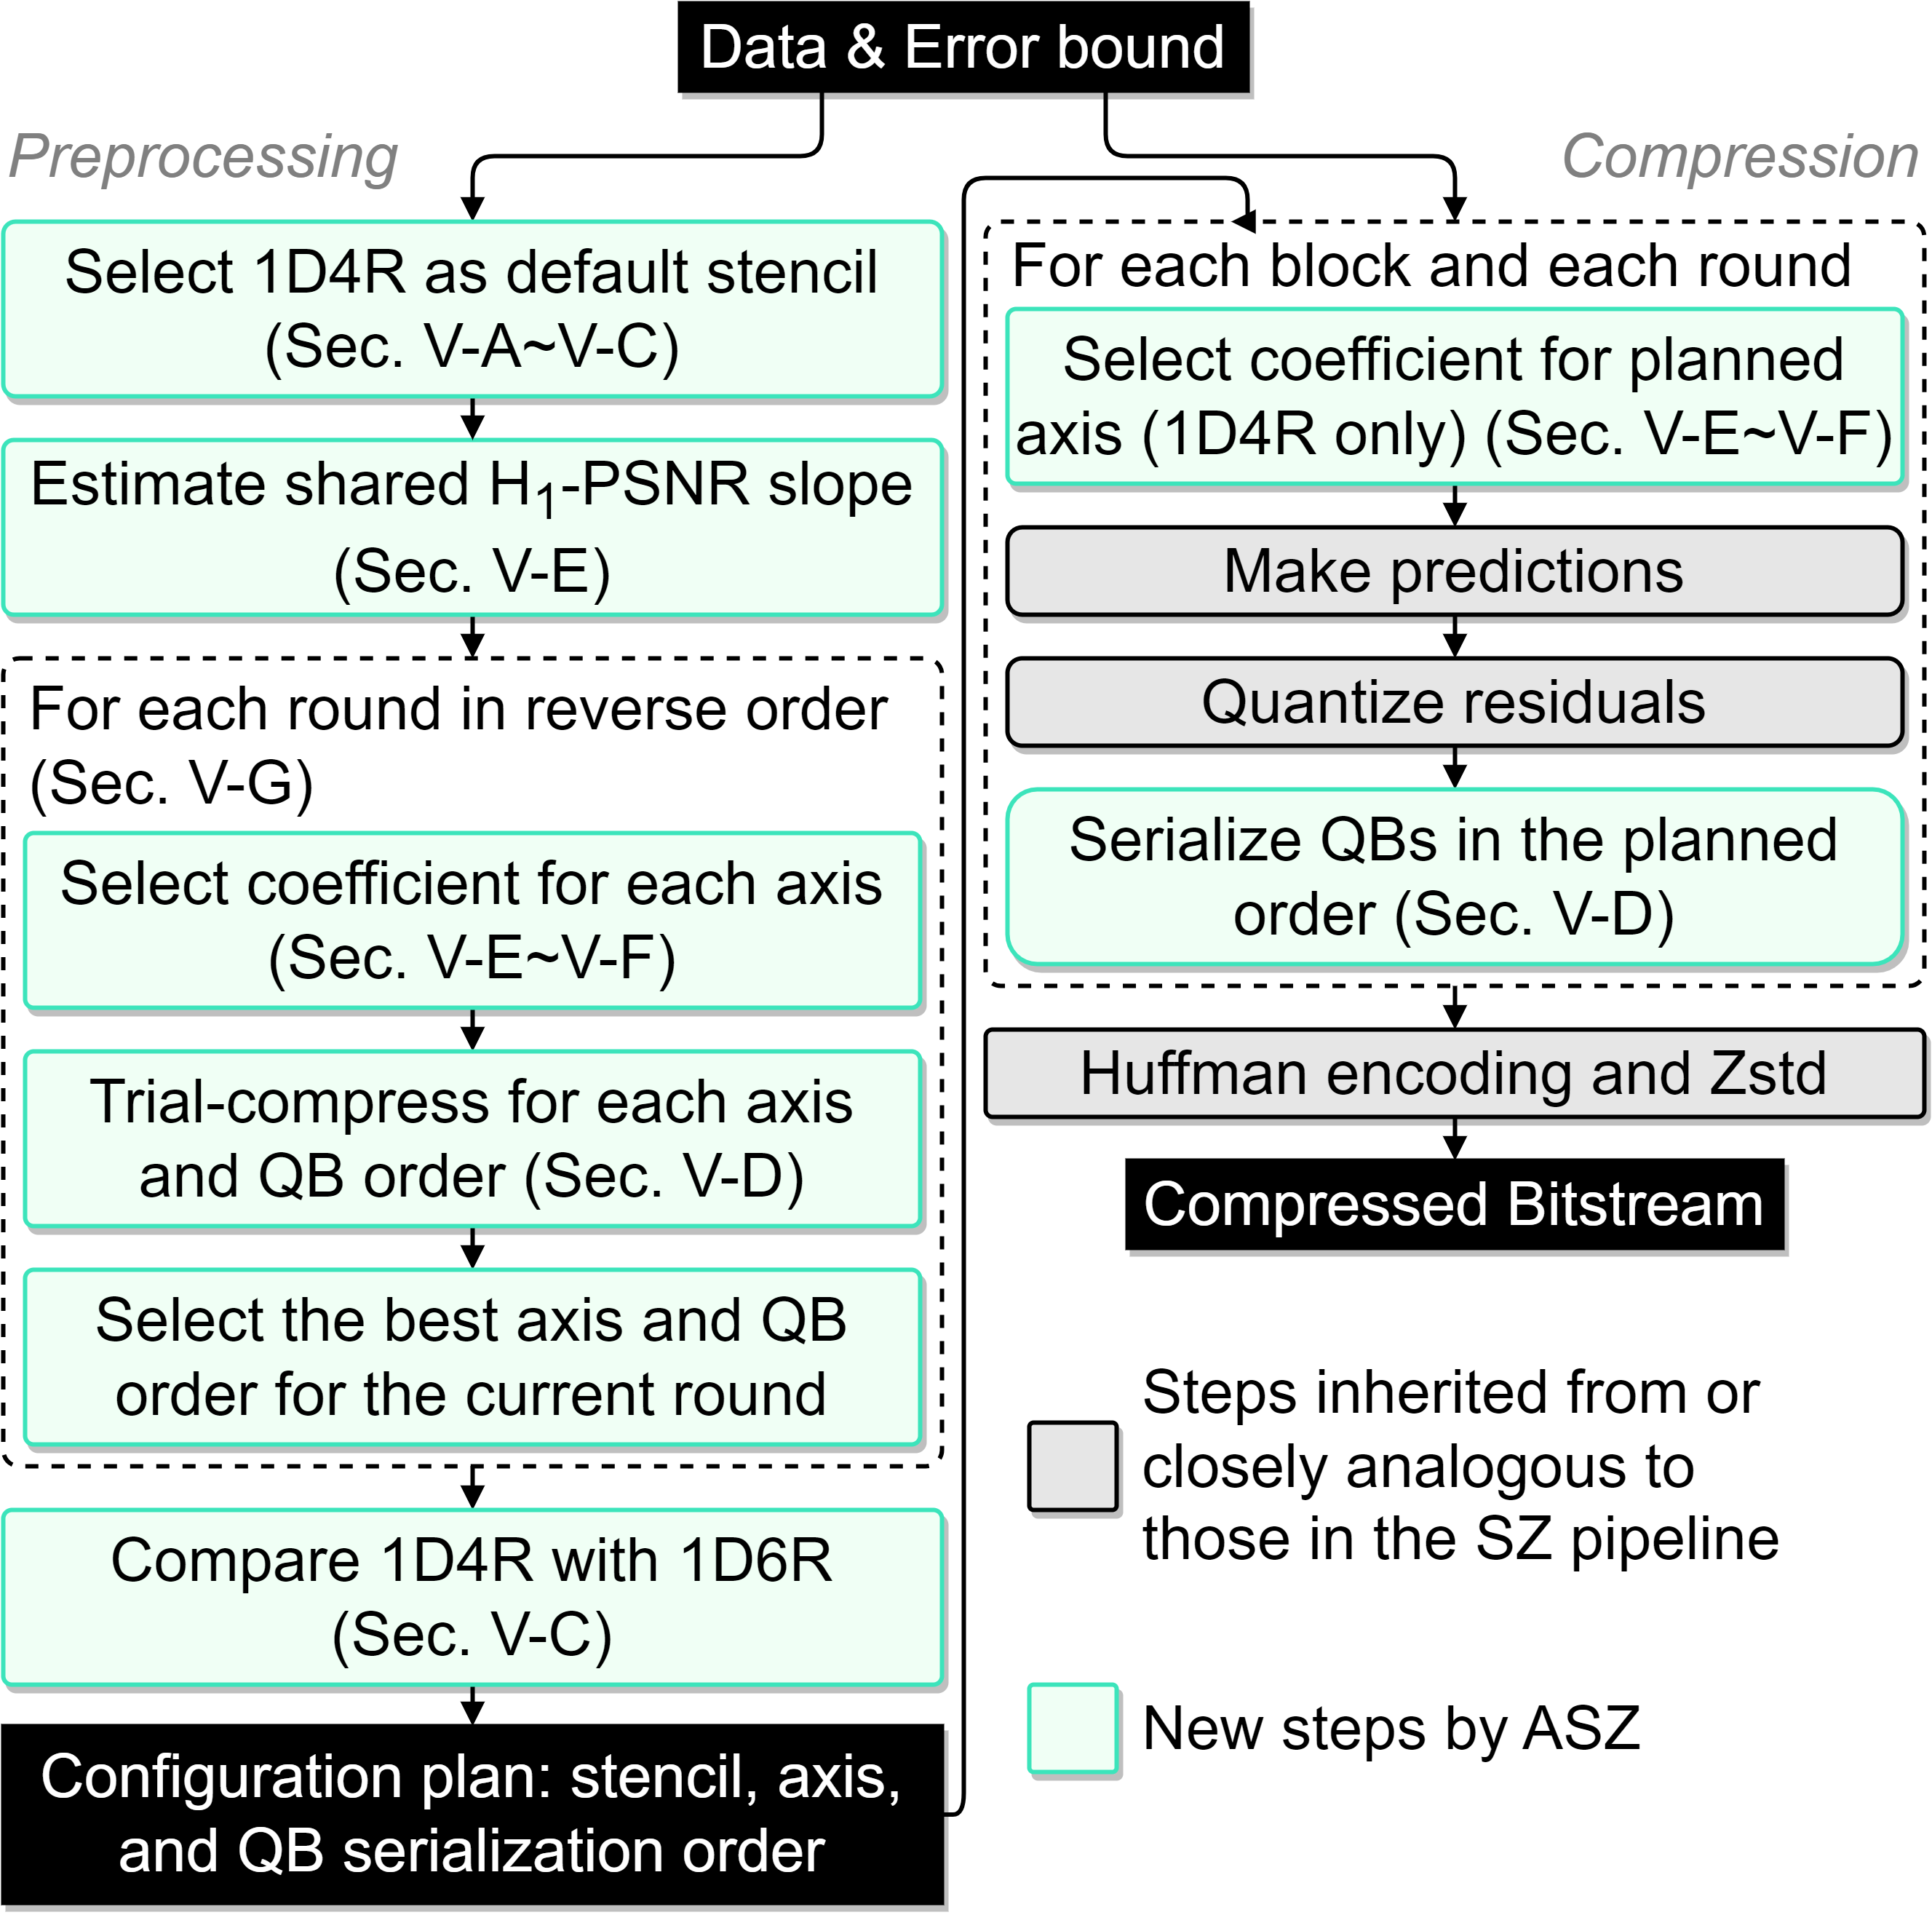
\includegraphics[width=\columnwidth]{revised-fig/asz_diagram.png}
\caption{ASZ workflow. Preprocessing constructs a configuration plan that specifies one prediction stencil for the entire field, together with one prediction axis and one QB serialization order for each round.}
\label{fig:overview:asz-workflow}
\end{figure}

\subsection{Overall Workflow and Configuration Reuse}
\label{sec:overview:plan-reuse}

ASZ generates the configuration plan $C_{\mathrm{reuse}}$ during preprocessing using the search and evaluation methods in Section~\ref{sec:optimization-strategies}. The plan can be generated for an individual input file or reused across related files to amortize preprocessing.

During compression, ASZ follows $C_{\mathrm{reuse}}$ and selects predictor coefficients separately for each block using a low-cost proxy.

\subsection{Round-Wise Configuration}
\label{sec:configuration-space:round-wise}

As Section~\ref{sec:background:configuration-granularity} shows, SZ3 and QoZ use each active axis once in every three-round cycle or group. Directional predictability, however, can differ across axes. For example, if a field is much smoother along $x$ than along $y$ and $z$, assigning more of the final rounds, which contain most targets, to $x$ can improve overall prediction accuracy. The once-per-group constraint rules out such schedules. ASZ therefore exposes the prediction axis and QB serialization order of every round as separate choices. Consecutive rounds may use the same axis, and the three axes may be selected different numbers of times. Fig.~\ref{fig:overview:round-schedules} contrasts the resulting per-round axis sequence with the configuration granularities of SZ3 and QoZ.

\begin{figure}[htb]
\centering
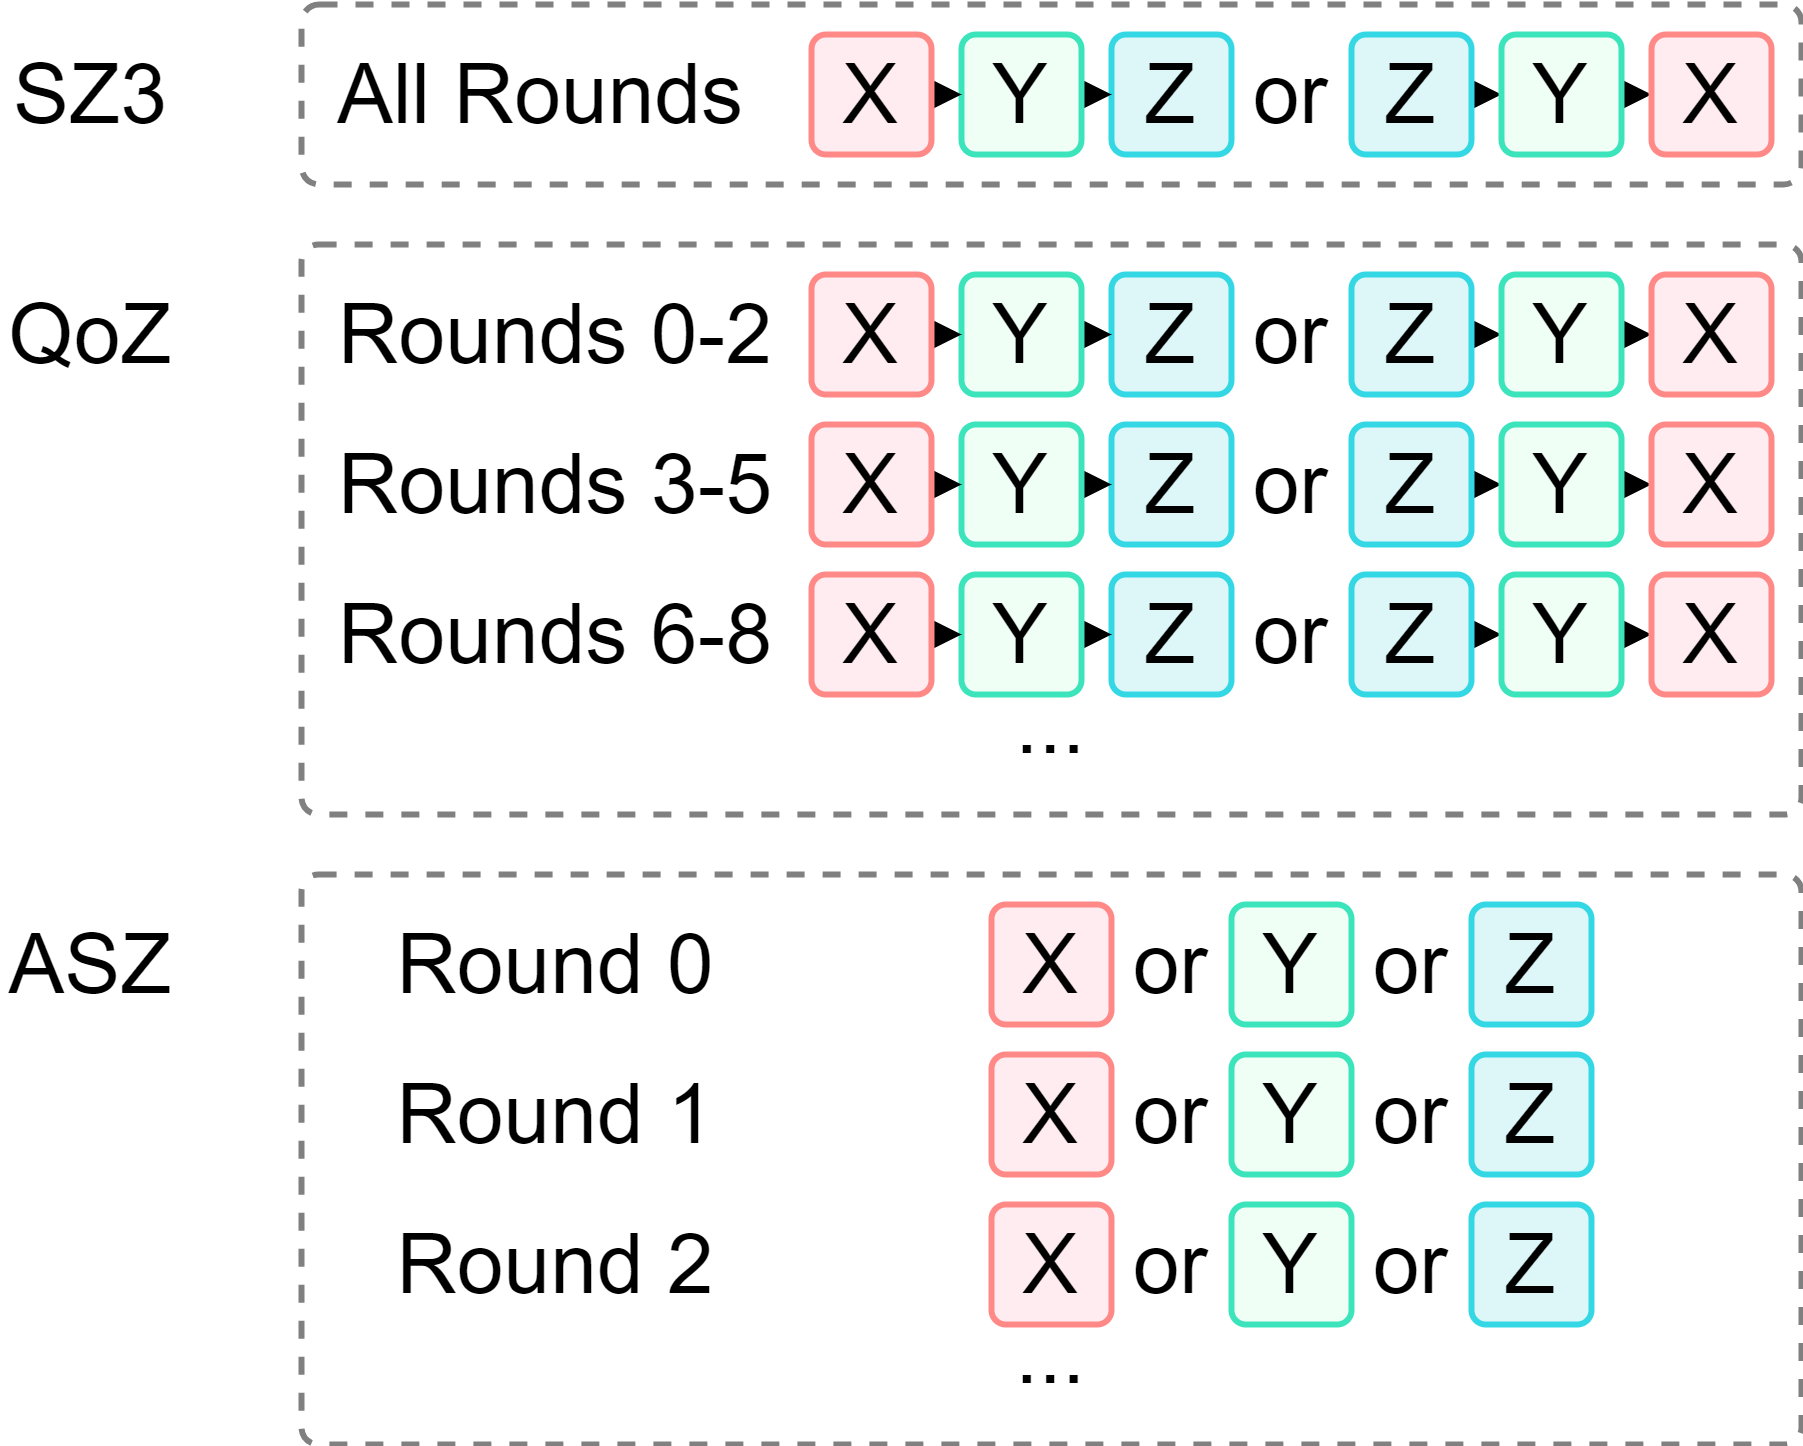
\includegraphics[width=.681818\linewidth]{revised-fig/configuration_granularity.png}
\caption{Prediction-axis configuration granularity for one-dimensional prediction on three-dimensional data. SZ3 selects a three-round cycle for the entire field, QoZ selects a cycle for each three-round group, and ASZ permits an unrestricted sequence of per-round axis choices. Boxes labeled X, Y, and Z denote prediction along the corresponding coordinate axes. The QB serialization order, which is fixed in SZ3 and QoZ but tuned separately for every ASZ round, is omitted.}
\label{fig:overview:round-schedules}
\end{figure}
